\begin{XeClass}{FtpFs}
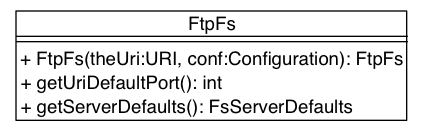
\includegraphics[width=\textwidth]{cdig/FtpFs.png}
     
 FTPFs是AbstractFileSystem以抽象的形式向Hadoop FS中具体的文件系统提供的实现接口
 DelegateToFileSystem是代理类
 FTPFs通过继承DelegateToFileSystem类,为旧式的文件系统提供了代理接口

    \begin{XeMethod}{}{FtpFs}{FtpFs}
         
 构造函数需要链接到上层抽象类AbstractFileSystem的URL和Configuration\emph{AbstractFileSystem.createFileSystem(URI,Configuration)}.

    \end{XeMethod}

    \begin{XeMethod}{\XeProtected}{int}{getUriDefaultPort}
         
 返回FTP的默认端口

    \end{XeMethod}

    \begin{XeMethod}{\XeProtected}{FsServerDefaults}{getServerDefaults}
         
 返回FtpConfigKeys类的getServerDefaults()方法的返回值,返回值是一个FsServerDefaults对象.

    \end{XeMethod}

\end{XeClass}
